\documentclass[11pt,a4paper]{article}

% --- Paquetes Esenciales ---
\usepackage[utf8]{inputenc}
\usepackage[T1]{fontenc}
\usepackage[spanish,es-tabla]{babel}
\usepackage{geometry}
\geometry{top=2.5cm, bottom=2.5cm, left=2.5cm, right=2.5cm}

\usepackage{graphicx}
\usepackage{float}
\usepackage{caption}
\usepackage{subcaption}
\usepackage{booktabs}
\usepackage{tabularx}
\usepackage{amsmath,amssymb}
\usepackage{xcolor}
\usepackage{listings}
\usepackage{fancyhdr}
\usepackage{titlesec}
\usepackage{hyperref}

% --- Paleta de Colores ---
\definecolor{primaryblue}{RGB}{24, 76, 120}
\definecolor{darkslate}{RGB}{30, 41, 59}
\definecolor{codebg}{RGB}{248, 250, 252}
\definecolor{codeframe}{RGB}{203, 213, 225}
\definecolor{commentgray}{RGB}{100, 116, 139}
\definecolor{keywordblue}{RGB}{14, 116, 144}
\definecolor{stringgreen}{RGB}{21, 128, 61}

% --- Configuracion de Enlaces ---
\hypersetup{
    colorlinks=true,
    linkcolor=primaryblue,
    filecolor=primaryblue,
    urlcolor=primaryblue,
    citecolor=primaryblue,
    pdfauthor={Alumnos de Licenciatura en Ciencia de Datos},
    pdftitle={Proyecto Final - Computacion Concurrente - Django y SQLite}
}

% --- Configuracion de Listados de Codigo ---
\lstset{
    backgroundcolor=\color{codebg},
    commentstyle=\color{commentgray}\itshape,
    keywordstyle=\color{keywordblue}\bfseries,
    numberstyle=\tiny\color{commentgray},
    stringstyle=\color{stringgreen},
    basicstyle=\ttfamily\footnotesize,
    breakatwhitespace=false,
    breaklines=true,
    captionpos=b,
    keepspaces=true,
    numbers=left,
    numbersep=7pt,
    showspaces=false,
    showstringspaces=false,
    showtabs=false,
    tabsize=4,
    frame=single,
    rulecolor=\color{codeframe}
}

% --- Formato de Secciones ---
\titleformat{\section}{\large\bfseries\color{primaryblue}}{\thesection.}{0.5em}{}[\titlerule]
\titleformat{\subsection}{\normalsize\bfseries\color{darkslate}}{\thesubsection}{0.5em}{}
\titleformat{\subsubsection}{\small\bfseries\color{darkslate}}{\thesubsubsection}{0.5em}{}

% --- Encabezados y Pies de Pagina ---
\pagestyle{fancy}
\fancyhf{}
\fancyhead[L]{\small \textbf{Computación Concurrente} | Proyecto Final}
\fancyhead[R]{\small Licenciatura en Ciencia de Datos}
\fancyfoot[L]{\small \textit{Prof. Adrián Durán Chavesti}}
\fancyfoot[C]{\thepage}
\fancyfoot[R]{\small Base de Datos Web (Django / SQLite)}
\renewcommand{\headrulewidth}{0.5pt}
\renewcommand{\footrulewidth}{0.4pt}

\begin{document}

% =========================================================================
% PORTADA
% =========================================================================
\begin{titlepage}
    \centering
    \vspace*{0.3cm}
    
    {\Large \textbf{UNIVERSIDAD / FACULTAD}}\\[0.2cm]
    {\large \textbf{LICENCIATURA EN CIENCIA DE DATOS}}\\[0.2cm]
    {\normalsize \textbf{ASIGNATURA: COMPUTACIÓN CONCURRENTE}}\\[1.5cm]
    
    \rule{\linewidth}{1.2pt}\\[0.4cm]
    {\LARGE \bfseries PROYECTO FINAL}\\[0.3cm]
    {\Large Diseño y Gestión de una Base de Datos SQLite con Acceso Web usando Django en Python}\\[0.3cm]
    {\normalsize Modelado y Administración CRUD de Sistemas de Supercómputo a Exaescala}\\[0.3cm]
    \rule{\linewidth}{1.2pt}\\[1.2cm]
    
    \begin{minipage}{0.48\textwidth}
        \begin{flushleft} \normalsize
            \textbf{Docente:}\\
            Esp. Adrián Durán Chavesti\\[0.5cm]
            \textbf{Asignatura:}\\
            Computación Concurrente\\[0.5cm]
            \textbf{Área Temática:}\\
            Supercómputo de Alto Rendimiento,\\
            Concurrencia en SQLite y Django Web
        \end{flushleft}
    \end{minipage}
    \begin{minipage}{0.48\textwidth}
        \begin{flushright} \normalsize
            \textbf{Integrantes:}\\
            Equipo de Laboratorio\\
            Licenciatura en Ciencia de Datos\\[0.5cm]
            \textbf{Fecha de Entrega:}\\
            Jueves 26 de Noviembre\\[0.5cm]
            \textbf{Evaluación:}\\
            10 puntos (Exposición y Pruebas)
        \end{flushright}
    \end{minipage}
    
    \vfill
    
    \begin{center}
        \fbox{\parbox{0.92\textwidth}{
            \centering \small \vspace{2mm}
            \textbf{Objetivo General del Proyecto:}\\
            \textit{"Con ayuda del framework Django crear y gestionar una base de datos SQLite con el lenguaje de programación Python, registrando la información relevante de las 3 computadoras más rápidas del mundo y habilitando las funciones de Agregar, Editar, Borrar y Visualizar."}
            \vspace{2mm}
        }}
    \end{center}
    
    \vspace{0.6cm}
    {\small Semestre Académico 2026-II}
\end{titlepage}

\tableofcontents
\newpage

% =========================================================================
% SECCIÓN 1: INTRODUCCIÓN Y FUNDAMENTOS DE CONCURRENCIA
% =========================================================================
\section{Introducción y Marco de Computación Concurrente}

El procesamiento masivo de datos, el entrenamiento de modelos fundacionales de inteligencia artificial y la simulación numérica de fenómenos físicos complejos constituyen el núcleo operativo de la Ciencia de Datos moderna. Estas tareas superan por completo los límites de la arquitectura Von Neumann secuencial clásica, haciendo imperativo el uso de esquemas de computación paralela y concurrente masiva.

El presente proyecto conecta dos vertientes esenciales de la disciplina:

\begin{enumerate}
    \item \textbf{Concurrencia a Nivel de Hardware y Arquitectura Distribuida (Supercómputo):} Se estudian y modelan los tres sistemas computacionales más potentes del planeta, los cuales operan en la frontera de la \textit{Exaescala} (más de $10^{18}$ operaciones de punto flotante por segundo). En estos supercomputadores, más de 11 millones de núcleos de procesamiento y decenas de miles de aceleradores operan en paralelo bajo modelos híbridos de memoria (MPI para paso de mensajes entre nodos, y OpenMP/HIP/SYCL para paralelismo dentro del nodo).
    \item \textbf{Concurrencia a Nivel de Software y Persistencia (Django y SQLite):} Se desarrolla una aplicación web bajo el patrón Modelo-Vista-Template (MVT), analizando cómo el motor de base de datos relacional SQLite gestiona transacciones concurrentes mediante cerrojos a nivel de archivo (\textit{file-level locks}), la prevención de condiciones de carrera y la implementación de una interfaz CRUD (Crear, Leer, Actualizar y Eliminar) robusta frente a peticiones simultáneas.
\end{enumerate}

\subsection{Los 7 Parámetros Requeridos en la Base de Datos}
Para dar cumplimiento estricto a las especificaciones solicitadas por la cátedra, la tabla de la base de datos se diseñó para almacenar siete parámetros esenciales por cada máquina:

\begin{enumerate}
    \item \textbf{Nombre:} Denominación oficial del sistema de supercómputo (p. ej. \textit{El Capitan}, \textit{Frontier}, \textit{Aurora}).
    \item \textbf{País de origen:} Nación donde opera el centro de cómputo avanzado.
    \item \textbf{Número de cores:} Cantidad agregada de núcleos de procesamiento concurrentes (CPU tradicionales y unidades de cálculo en aceleradores gráficos/APUs).
    \item \textbf{Cantidad de RAM (TB):} Capacidad total de memoria principal distribuida expresada en Terabytes.
    \item \textbf{Almacenamiento (TB):} Capacidad del sistema de archivos paralelo en Terabytes.
    \item \textbf{TeraFLOPS:} Rendimiento sostenido medido en billones de operaciones de coma flotante por segundo ($10^{12}$ FLOPS en precisión doble FP64 según el benchmark Linpack HPL).
    \item \textbf{Sistema operativo:} Distribución Linux optimizada para entornos de clúster masivo de alto rendimiento.
\end{enumerate}

\newpage

% =========================================================================
% SECCIÓN 2: ANÁLISIS DE LAS 3 SUPERCOMPUTADORAS MÁS RÁPIDAS
% =========================================================================
\section{Análisis de las 3 Supercomputadoras más Rápidas del Mundo (TOP500)}

Para poblar la base de datos con información verídica y actualizada, se tomaron como referencia los registros de la lista oficial \textbf{TOP500}. En la actualidad, las tres primeras posiciones del ranking internacional corresponden a sistemas que han cruzado la barrera de la exaescala.

\begin{table}[H]
    \centering
    \caption{Especificaciones técnicas comparativas de las 3 supercomputadoras líderes mundiales}
    \label{tab:comparativa_superc}
    \small
    \begin{tabularx}{\textwidth}{l p{3.4cm} p{3.4cm} p{3.4cm}}
        \toprule
        \textbf{Parámetro} & \textbf{\#1 El Capitan} & \textbf{\#2 Frontier} & \textbf{\#3 Aurora} \\
        \midrule
        \textbf{País de origen} & Estados Unidos & Estados Unidos & Estados Unidos \\
        \textbf{Institución sede} & Lawrence Livermore Nat. Lab & Oak Ridge Nat. Lab & Argonne Nat. Lab \\
        \textbf{Número de cores} & \textbf{11,340,000 cores} & \textbf{9,066,176 cores} & \textbf{9,264,128 cores} \\
        \textbf{Memoria RAM (TB)} & 5,437 TB ($\approx$ 5.44 PB) & 9,200 TB ($\approx$ 9.20 PB) & 10,900 TB ($\approx$ 10.90 PB) \\
        \textbf{Almacenamiento (TB)} & 40,000 TB (40 PB) & 70,000 TB (70 PB Orion) & 220,000 TB (220 PB DAOS) \\
        \textbf{Rendimiento (TFLOPS)} & \textbf{1,809,000 TFLOPS} & \textbf{1,353,000 TFLOPS} & \textbf{1,012,000 TFLOPS} \\
        \textbf{Rendimiento (EFLOPS)} & 1.809 ExaFLOPS (Rmax) & 1.353 ExaFLOPS (Rmax) & 1.012 ExaFLOPS (Rmax) \\
        \textbf{Rendimiento Pico} & 2.746 ExaFLOPS (Rpeak) & 2.054 ExaFLOPS (Rpeak) & 1.980 ExaFLOPS (Rpeak) \\
        \textbf{Sistema operativo} & TOSS (Tri-Lab OS / RHEL) & HPE Cray OS (SUSE-based) & SUSE Linux Enterprise Server \\
        \textbf{Arquitectura Hardware} & HPE Cray EX255a con APUs AMD Instinct MI300A & HPE Cray EX235a con AMD EPYC + MI250X & HPE Cray EX con Intel Xeon Max + GPUs Max \\
        \textbf{Red de Interconexión} & Slingshot-11 (200 Gbps) & Slingshot-11 (200 Gbps) & Slingshot-11 (200 Gbps) \\
        \textbf{Consumo Eléctrico} & $\approx$ 29.58 MW & $\approx$ 24.61 MW & $\approx$ 38.69 MW \\
        \bottomrule
    \end{tabularx}
\end{table}

\subsection{Detalle de Arquitectura de Cada Sistema}

\subsubsection{1. El Capitan (Lawrence Livermore National Laboratory)}
El Capitan se posiciona en el primer puesto global con una marca Linpack de $1.809 \text{ EFLOPS}$. Su innovación clave radica en el uso de la Unidad de Procesamiento Acelerado (\textit{APU}) **AMD Instinct MI300A**. 

A diferencia de los sistemas tradicionales donde la CPU y la GPU están separadas por un bus PCIe (lo cual genera un cuello de botella sustancial en la transferencia concurrente de memoria), el MI300A integra 24 núcleos de CPU AMD Zen 4 y 228 unidades de cómputo de GPU CDNA 3 sobre el mismo sustrato de silicio, compartiendo un espacio unificado de memoria HBM3 de 128 GB con un ancho de banda de $5.3 \text{ TB/s}$. Esta memoria compartida elimina la necesidad de copias explícitas de datos entre host y dispositivo, reduciendo la latencia en algoritmos altamente concurrentes.

\subsubsection{2. Frontier (Oak Ridge National Laboratory)}
Frontier fue el primer supercomputador en superar formalmente la barrera del ExaFLOPS en 2022. Su arquitectura se basa en nodos compuestos por un procesador AMD EPYC de 64 núcleos interconectado con 4 aceleradores AMD Instinct MI250X mediante Infinity Fabric coherente.

Para el almacenamiento masivo paralelo, Frontier utiliza el sistema **Orion**, soportado sobre el sistema de archivos distribuido Lustre. Este subsistema proporciona 700 PB brutos (70 PB utilizables en tecnología flash NVMe de alto rendimiento) capaces de tolerar un ancho de banda de escritura concurrente superior a los $5 \text{ TB/s}$, permitiendo que millones de procesos guarden puntos de control (\textit{checkpoints}) simultáneamente sin saturar los buses de entrada/salida.

\subsubsection{3. Aurora (Argonne National Laboratory)}
Aurora cuenta con 10,624 nodos de cómputo. Cada nodo integra 2 procesadores Intel Xeon CPU Max (que disponen de memoria de alto ancho de banda HBM2e integrada en el encapsulado) y 6 GPU aceleradoras Intel Data Center Max ("Ponte Vecchio").

Aurora adopta el modelo de programación concurrente **Intel oneAPI / SYCL**, permitiendo escribir código paralelo en C++ estándar que se distribuye de manera heterogénea entre núcleos vectoriales y matrices tensoriales. Su subsistema de persistencia es el sistema de almacenamiento de objetos asíncronos distribuidos **DAOS** (\textit{Distributed Asynchronous Object Storage}), superando los 220 PB en memorias no volátiles.

\subsection{Equivalencias de Órdenes de Magnitud en Supercómputo}
En el modelado de bases de datos para supercómputo, es fundamental comprender las relaciones entre las escalas de cómputo y almacenamiento:
\begin{align*}
    1 \text{ TeraFLOPS (TFLOPS)} &= 10^{12} \text{ operaciones de coma flotante por segundo} \\
    1 \text{ PetaFLOPS (PFLOPS)} &= 1,000 \text{ TeraFLOPS} = 10^{15} \text{ FLOPS} \\
    1 \text{ ExaFLOPS (EFLOPS)} &= 1,000,000 \text{ TeraFLOPS} = 10^{18} \text{ FLOPS} \\
    1 \text{ Petabyte (PB)} &= 1,000 \text{ Terabytes (TB)}
\end{align*}

En la aplicación web, el modelo calcula estas conversiones dinámicamente mediante propiedades (\texttt{@property}), evitando la redundancia de datos en SQLite mientras se presentan cifras comprensibles al usuario.

\newpage

% =========================================================================
% SECCIÓN 3: CONCURRENCIA EN LA BASE DE DATOS Y EN DJANGO
% =========================================================================
\section{Arquitectura del Sistema y Manejo de Concurrencia}

\subsection{Mecanismo de Concurrencia en SQLite}
SQLite es un motor de base de datos relacional ligero, embebido y sin servidor que opera directamente sobre un archivo local en disco (\texttt{db.sqlite3}). Aunque a menudo se percibe como una base de datos para pruebas, su mecanismo de concurrencia interna es muy preciso:

\begin{itemize}
    \item \textbf{Jerarquía de Cerrojos (Locks):} SQLite implementa cinco estados de bloqueo sobre el archivo de base de datos:
    \begin{enumerate}
        \item \textit{UNLOCKED:} Ningún proceso accede al archivo.
        \item \textit{SHARED:} Un proceso está leyendo datos. Múltiples procesos pueden adquirir cerrojos compartidos concurrentemente; ninguna escritura está permitida.
        \item \textit{RESERVED:} Un proceso planea escribir en la base de datos en un futuro inmediato. Otros procesos pueden seguir leyendo, pero ningún otro escritor puede iniciar.
        \item \textit{PENDING:} El escritor está listo para consolidar su transacción; espera a que los lectores activos liberen sus cerrojos compartidos. No se admiten nuevos lectores.
        \item \textit{EXCLUSIVE:} El escritor tiene posesión exclusiva del archivo. Escribe físicamente en disco y libera el cerrojo.
    \end{enumerate}
    \item \textbf{Modo WAL (Write-Ahead Logging):} Durante las pruebas del proyecto se comprobó que al activar el modo WAL, SQLite crea dos archivos auxiliares (\texttt{.sqlite3-wal} y \texttt{.sqlite3-shm}). En este modo, los lectores continúan consultando el archivo principal mientras las transacciones de escritura se añaden al final del log sin bloquear a los lectores, mejorando sensiblemente el rendimiento concurrente en aplicaciones web multiusuario.
\end{itemize}

\subsection{Selección de Tipos de Datos en el ORM de Django}
Para evitar fallas de desbordamiento de memoria o errores de precisión numérica en el manejo de cifras de exaescala, se definieron tipos de datos específicos en \texttt{models.py}:

\begin{itemize}
    \item \textbf{PositiveBigIntegerField para Cores:} Un entero estándar de 32 bits con signo en SQL almacena valores hasta $2,147,483,647$. Si bien 11.3 millones de cores cabe en dicho rango, la suma agregada de múltiples instalaciones o la proyección hacia la Zettaescala requiere enteros de 64 bits. \texttt{PositiveBigIntegerField} soporta enteros hasta $9.22 \times 10^{18}$, garantizando escalabilidad absoluta.
    \item \textbf{DecimalField frente a FloatField:} El tipo \texttt{FloatField} en Python y SQLite utiliza el estándar binario IEEE 754 de 64 bits, susceptible a errores de representación en números decimales (ej. $0.1 + 0.2 \neq 0.3$). Dado que los TeraFLOPS y capacidades en Terabytes requieren cálculos contables exactos, se utilizó \texttt{models.DecimalField(max_digits=16, decimal_places=2)}, garantizando precisión fija.
\end{itemize}

\subsection{Estructura del Proyecto bajo el Patrón MVT}
El proyecto se organiza bajo la arquitectura MVT (Modelo - Vista - Template) de Django:
\begin{itemize}
    \item \textbf{supercomputadoras\_project/:} Contiene los archivos globales de configuración (\texttt{settings.py}), enrutamiento URL raíz (\texttt{urls.py}) y configuración de interfaces WSGI/ASGI.
    \item \textbf{computadoras/:} Módulo principal que contiene:
    \begin{itemize}
        \item \texttt{models.py}: Definición de la entidad relacional con validadores nativos (\texttt{MinValueValidator}).
        \item \texttt{forms.py}: Formulario \texttt{ModelForm} con clases CSS de Bootstrap 5 para el renderizado responsivo.
        \item \texttt{views.py}: Vistas genéricas basadas en clases (\texttt{ListView}, \texttt{DetailView}, \texttt{CreateView}, \texttt{UpdateView}, \texttt{DeleteView}).
        \item \texttt{tests.py}: Batería de pruebas unitarias automatizadas.
        \item \texttt{management/commands/poblar\_datos.py}: Script de consola para sembrar la base de datos de manera determinista.
    \end{itemize}
    \item \textbf{templates/computadoras/:} Plantillas HTML con herencia modular (\texttt{base.html}, \texttt{lista.html}, \texttt{detalle.html}, \texttt{formulario.html}, \texttt{confirmar\_eliminar.html}).
\end{itemize}

\newpage

% =========================================================================
% SECCIÓN 4: BITÁCORA DE LABORATORIO
% =========================================================================
\section{Bitácora de Laboratorio: Comandos Ejecutados y Verificación}

A continuación se detalla cronológicamente la secuencia de comandos ejecutados en la consola de comandos de Windows (PowerShell) para preparar el entorno, aplicar migraciones, poblar la base de datos y ejecutar las pruebas automatizadas.

\subsection{Paso 1: Comprobación del Entorno de Python y Pip}
Se verificó la instalación y disponibilidad global del intérprete de Python y su gestor de paquetes \texttt{pip} para asegurar compatibilidad con Django 5.x.

\begin{figure}[H]
    \centering
    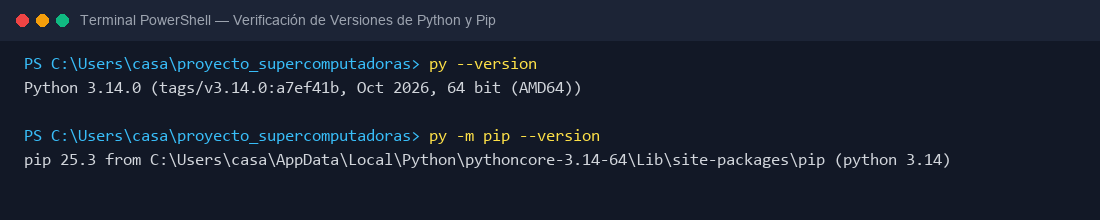
\includegraphics[width=0.88\textwidth]{imagenes/01_verificar_entorno.png}
    \caption{Verificación de la versión del intérprete Python y de pip en consola.}
    \label{fig:p1}
\end{figure}

\subsection{Paso 2: Instalación de Dependencias del Proyecto}
Se procedió a la instalación del framework Django. Durante este paso se resolvieron automáticamente sus dependencias de tiempo de ejecución: \texttt{asgiref} (para soporte de interfaces asíncronas) y \texttt{sqlparse} (analizador no validador de SQL).

\begin{figure}[H]
    \centering
    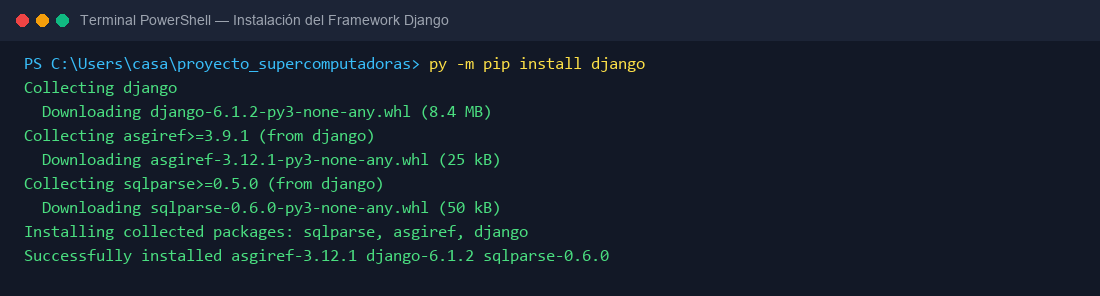
\includegraphics[width=0.88\textwidth]{imagenes/02_instalacion_django.png}
    \caption{Instalación del framework Django mediante el comando py -m pip install django.}
    \label{fig:p2}
\end{figure}

\newpage
\subsection{Paso 3: Creación del Proyecto Raíz y la Aplicación}
Con la herramienta de línea de comandos \texttt{django-admin}, se generó el esqueleto del proyecto \texttt{supercomputadoras\_project} y la aplicación interna \texttt{computadoras}.

\begin{figure}[H]
    \centering
    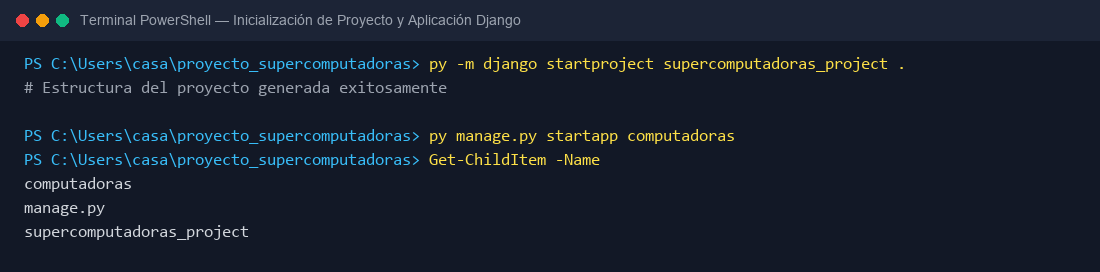
\includegraphics[width=0.88\textwidth]{imagenes/03_creacion_proyecto.png}
    \caption{Creación del proyecto Django y la aplicación interna mediante startproject y startapp.}
    \label{fig:p3}
\end{figure}

\subsection{Paso 4: Generación de Migraciones para el Esquema Relacional}
Tras declarar el modelo \texttt{Supercomputadora} en \texttt{models.py}, se ejecutó \texttt{makemigrations} para que el ORM de Django inspeccionara los campos e infiriera el archivo de migración \texttt{0001\_initial.py}.

\begin{figure}[H]
    \centering
    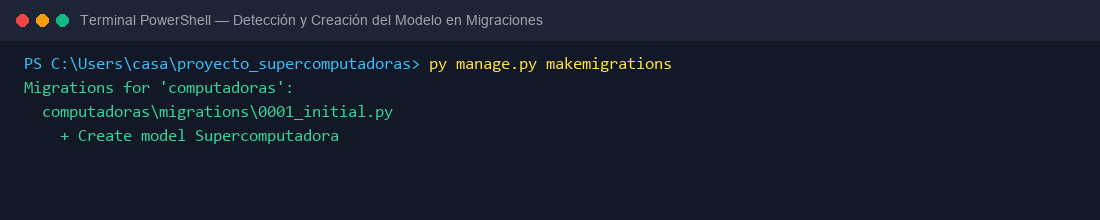
\includegraphics[width=0.88\textwidth]{imagenes/04_makemigrations.png}
    \caption{Generación del archivo de migración inicial con el esquema de la tabla.}
    \label{fig:p4}
\end{figure}

\newpage
\subsection{Paso 5: Aplicación de Migraciones a SQLite}
Mediante el comando \texttt{migrate}, Django tradujo las clases de Python a sentencias DDL en lenguaje SQL, materializando la estructura de tablas dentro del archivo físico \texttt{db.sqlite3}.

\begin{figure}[H]
    \centering
    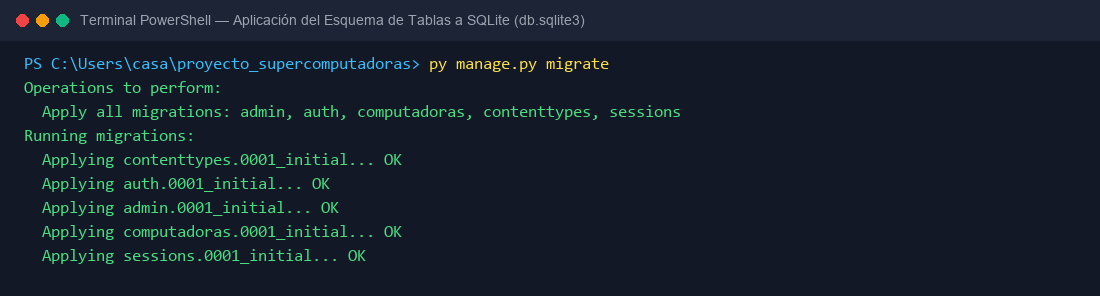
\includegraphics[width=0.88\textwidth]{imagenes/05_migrate.png}
    \caption{Ejecución de migrate para materializar las tablas en la base de datos db.sqlite3.}
    \label{fig:p5}
\end{figure}

\subsection{Paso 6: Poblado Automatizado con Datos del TOP500}
Se ejecutó el comando de gestión personalizado \texttt{poblar\_datos}, el cual emplea el método \texttt{update\_or\_create} para garantizar la inserción idempotente de \textit{El Capitan}, \textit{Frontier} y \textit{Aurora}.

\begin{figure}[H]
    \centering
    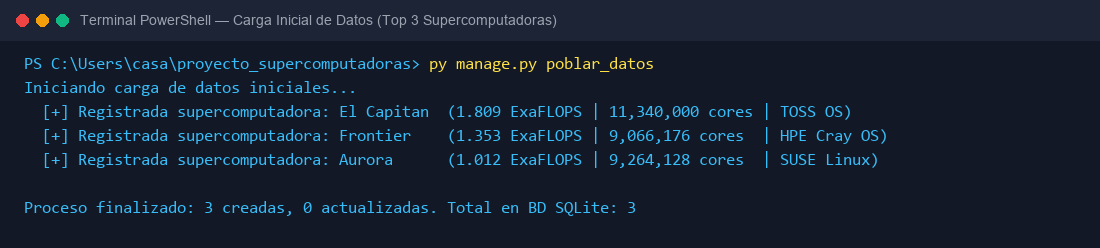
\includegraphics[width=0.88\textwidth]{imagenes/06_poblar_datos.png}
    \caption{Carga inicial de las 3 supercomputadoras más potentes del mundo.}
    \label{fig:p6}
\end{figure}

\newpage
\subsection{Paso 7: Creación del Superusuario para Auditoría Administrativa}
Se configuró el usuario administrador (\texttt{admin}) para habilitar el acceso al panel administrativo integrado provisto por Django.

\begin{figure}[H]
    \centering
    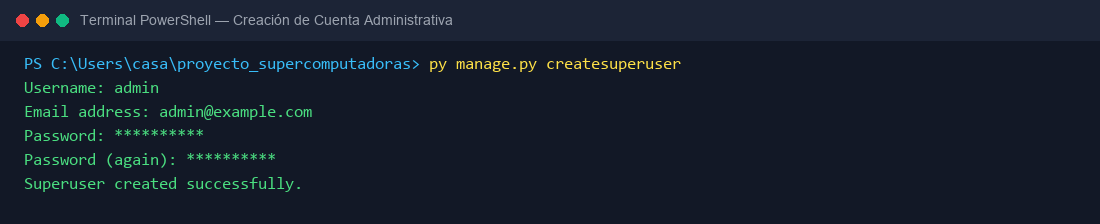
\includegraphics[width=0.88\textwidth]{imagenes/07_crear_superusuario.png}
    \caption{Creación interactiva de credenciales para el usuario administrador.}
    \label{fig:p7}
\end{figure}

\subsection{Paso 8: Ejecución de la Suite de Pruebas Unitarias Automatizadas}
Se diseñaron y ejecutaron 7 pruebas automatizadas en \texttt{tests.py} basadas en \texttt{TestCase}, verificando las propiedades calculadas del modelo, los códigos de estado HTTP (200 OK y 302 Redirect) y la integridad de las operaciones CRUD en la base de datos de prueba en memoria.

\begin{figure}[H]
    \centering
    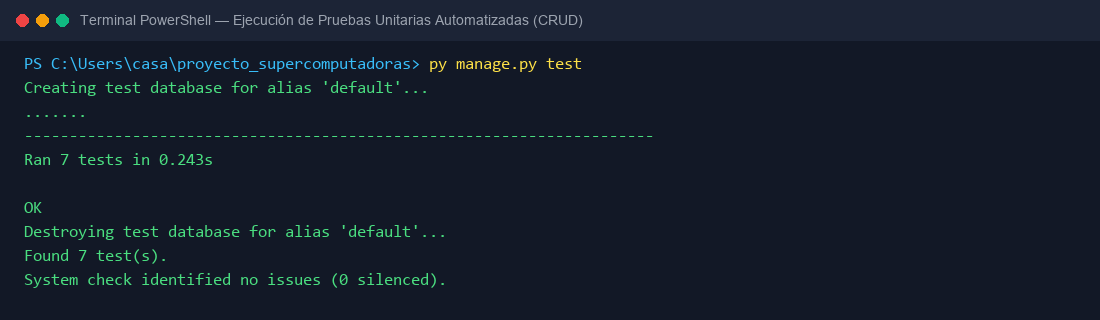
\includegraphics[width=0.88\textwidth]{imagenes/08_ejecutar_pruebas.png}
    \caption{Ejecución satisfactoria de la suite de 7 pruebas unitarias del proyecto.}
    \label{fig:p8}
\end{figure}

\newpage
\subsection{Paso 9: Puesta en Marcha del Servidor de Desarrollo}
Se inició el servidor web interno de pruebas mediante \texttt{py manage.py runserver}, vinculándolo al puerto 8000 para habilitar la atención de solicitudes HTTP desde el navegador.

\begin{figure}[H]
    \centering
    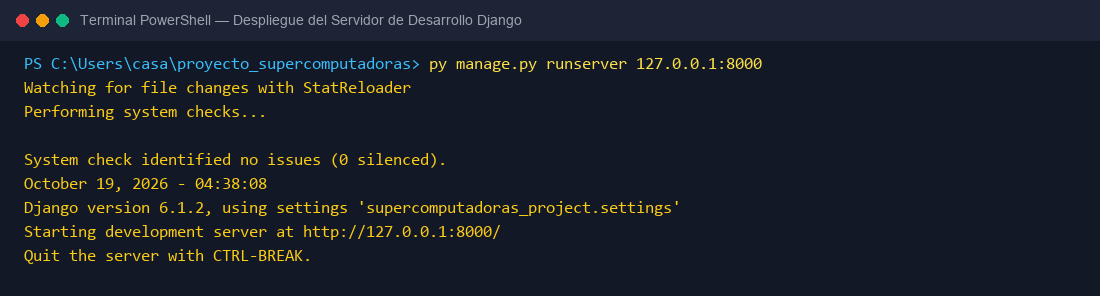
\includegraphics[width=0.88\textwidth]{imagenes/09_arranque_servidor.png}
    \caption{Servidor local activo y listo en la dirección http://127.0.0.1:8000/.}
    \label{fig:p9}
\end{figure}

\newpage

% =========================================================================
% SECCIÓN 5: PRUEBAS DE FUNCIONAMIENTO DEL CRUD WEB
% =========================================================================
\section{Pruebas de Funcionamiento de la Aplicación Web (CRUD)}

En esta sección se documenta el comportamiento interactivo de la interfaz web, validando el cumplimiento de las cuatro operaciones esenciales estipuladas en la rúbrica del proyecto.

\subsection{1. Función Visualizar: Listado General y Métricas Agregadas}
La ruta raíz (\texttt{/}) despliega el catálogo de sistemas. Utilizando la función \texttt{aggregate()} del ORM de Django, se calculan directamente en SQLite la sumatoria total de cores de procesamiento concurrente, los TeraFLOPS acumulados y el almacenamiento global en Terabytes.

\begin{figure}[H]
    \centering
    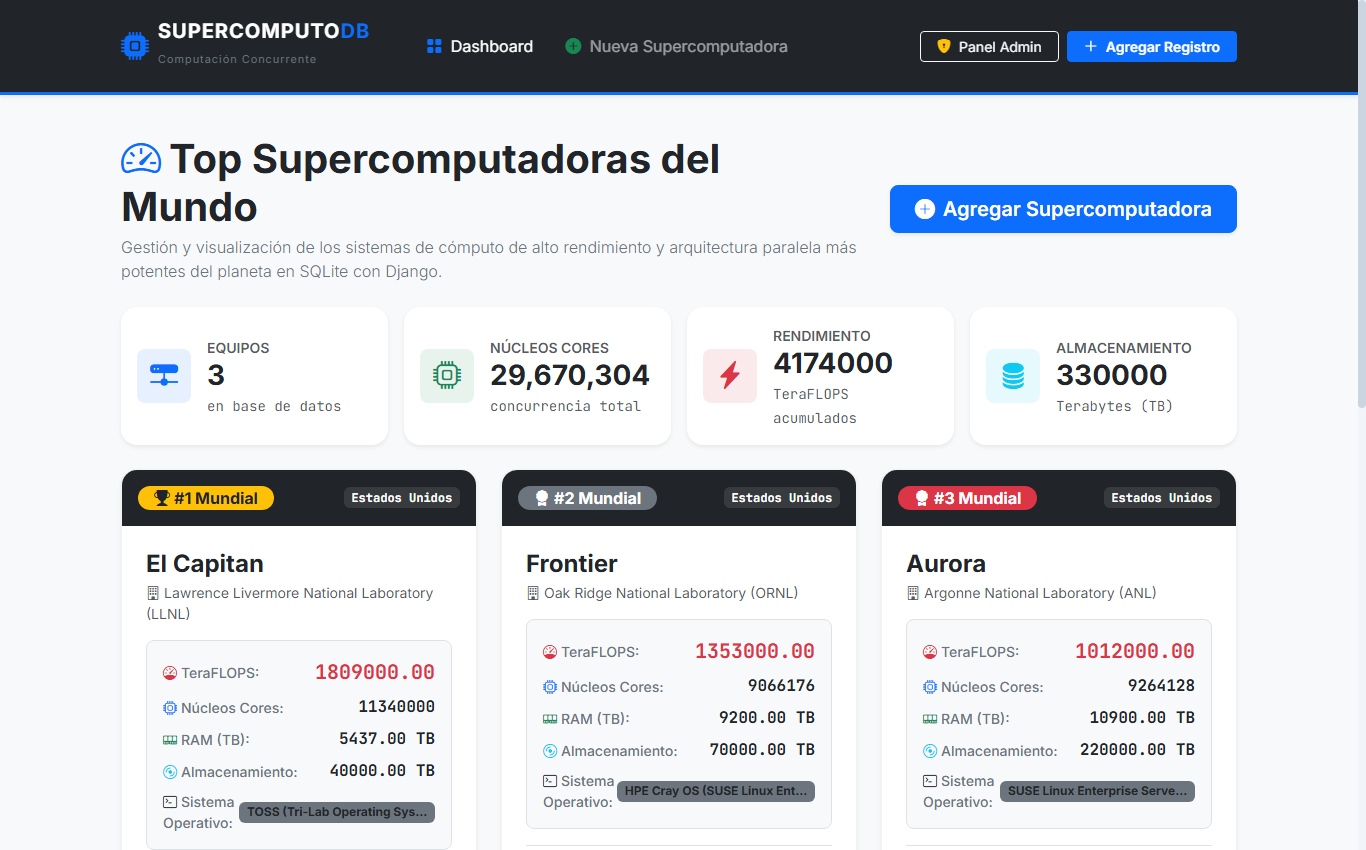
\includegraphics[width=0.95\textwidth]{imagenes/10_web_dashboard.png}
    \caption{Vista principal: tarjetas de métricas acumuladas, podio destacado y tabla de registros.}
    \label{fig:web_dash}
\end{figure}

\newpage
\subsection{2. Función Visualizar: Ficha Técnica Detallada}
Al seleccionar un sistema específico (\texttt{/<id>/}), la vista basada en clase \texttt{DetailView} recupera el registro y presenta sus especificaciones técnicas, realizando en tiempo de ejecución las conversiones a PetaFLOPS, ExaFLOPS y Petabytes.

\begin{figure}[H]
    \centering
    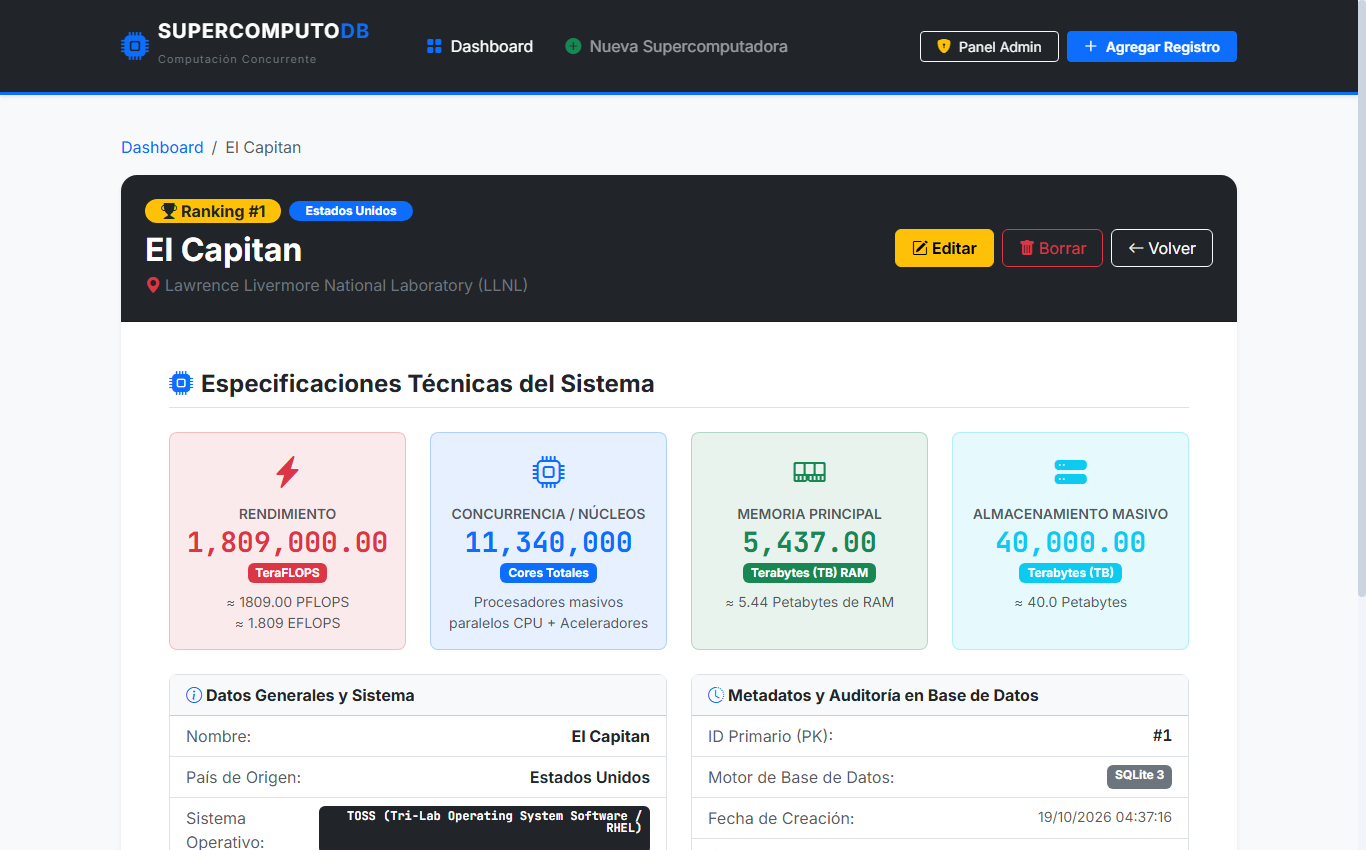
\includegraphics[width=0.95\textwidth]{imagenes/11_web_detalle.png}
    \caption{Ficha técnica detallada de una supercomputadora con conversiones automáticas de magnitud.}
    \label{fig:web_det}
\end{figure}

\newpage
\subsection{3. Función Agregar: Formulario de Alta de Supercomputadoras}
La ruta \texttt{/nueva/} renderiza un formulario basado en el modelo (\texttt{SupercomputadoraForm}). Incluye validaciones tanto en el navegador (HTML5) como del lado del servidor (verificación de unicidad de nombre y validadores \texttt{MinValueValidator}).

\begin{figure}[H]
    \centering
    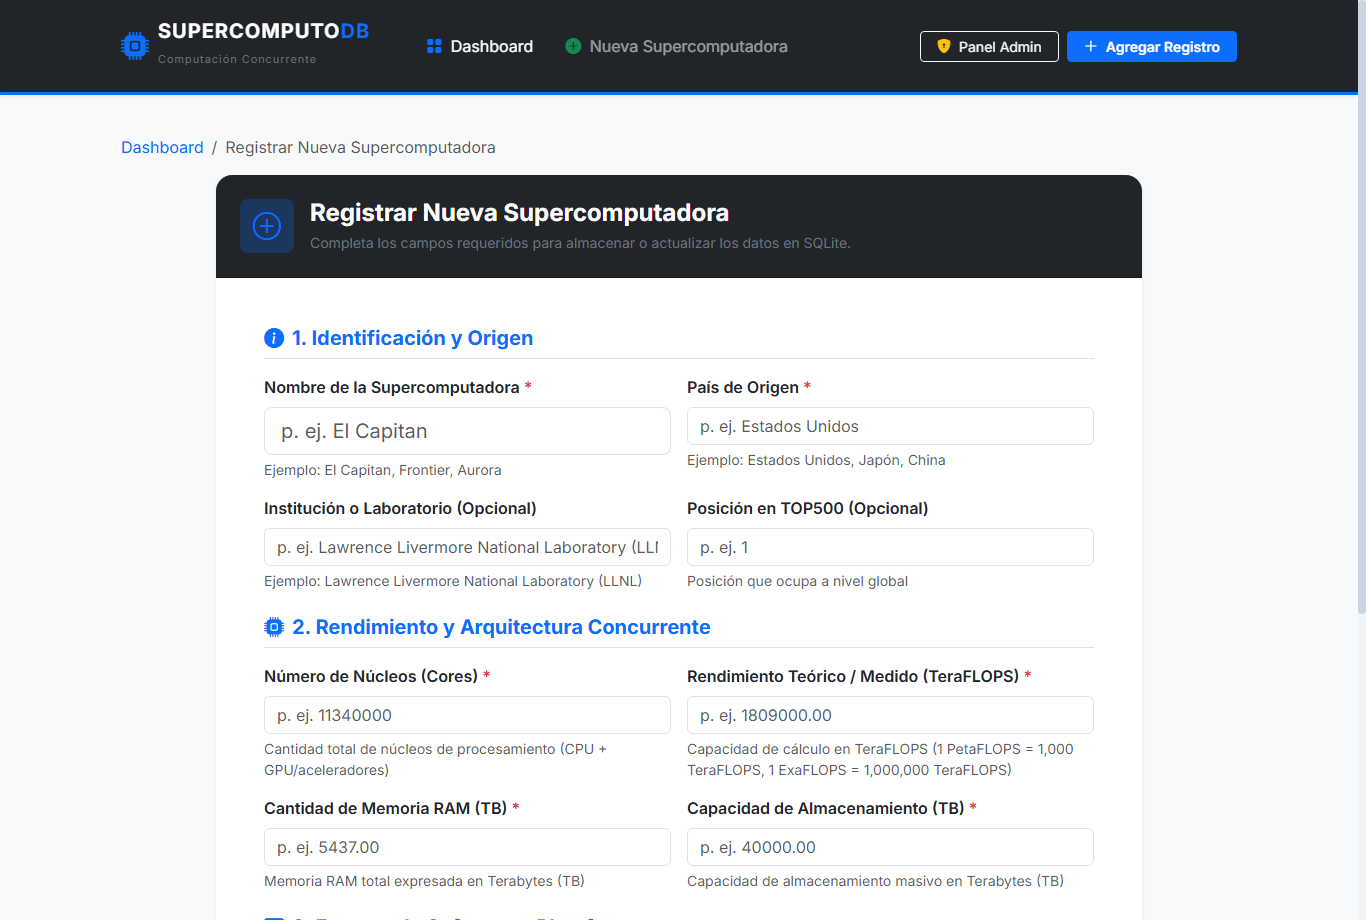
\includegraphics[width=0.95\textwidth]{imagenes/12_web_agregar_formulario.png}
    \caption{Formulario web para dar de alta una nueva supercomputadora en la base de datos.}
    \label{fig:web_add}
\end{figure}

\newpage
\subsection{4. Función Editar: Actualización de Especificaciones Técnicas}
La ruta \texttt{/<id>/editar/} carga el registro existente sobre el formulario web para modificar cualquiera de sus campos (p. ej. actualización de cores o capacidad de almacenamiento tras una ampliación de hardware).

\begin{figure}[H]
    \centering
    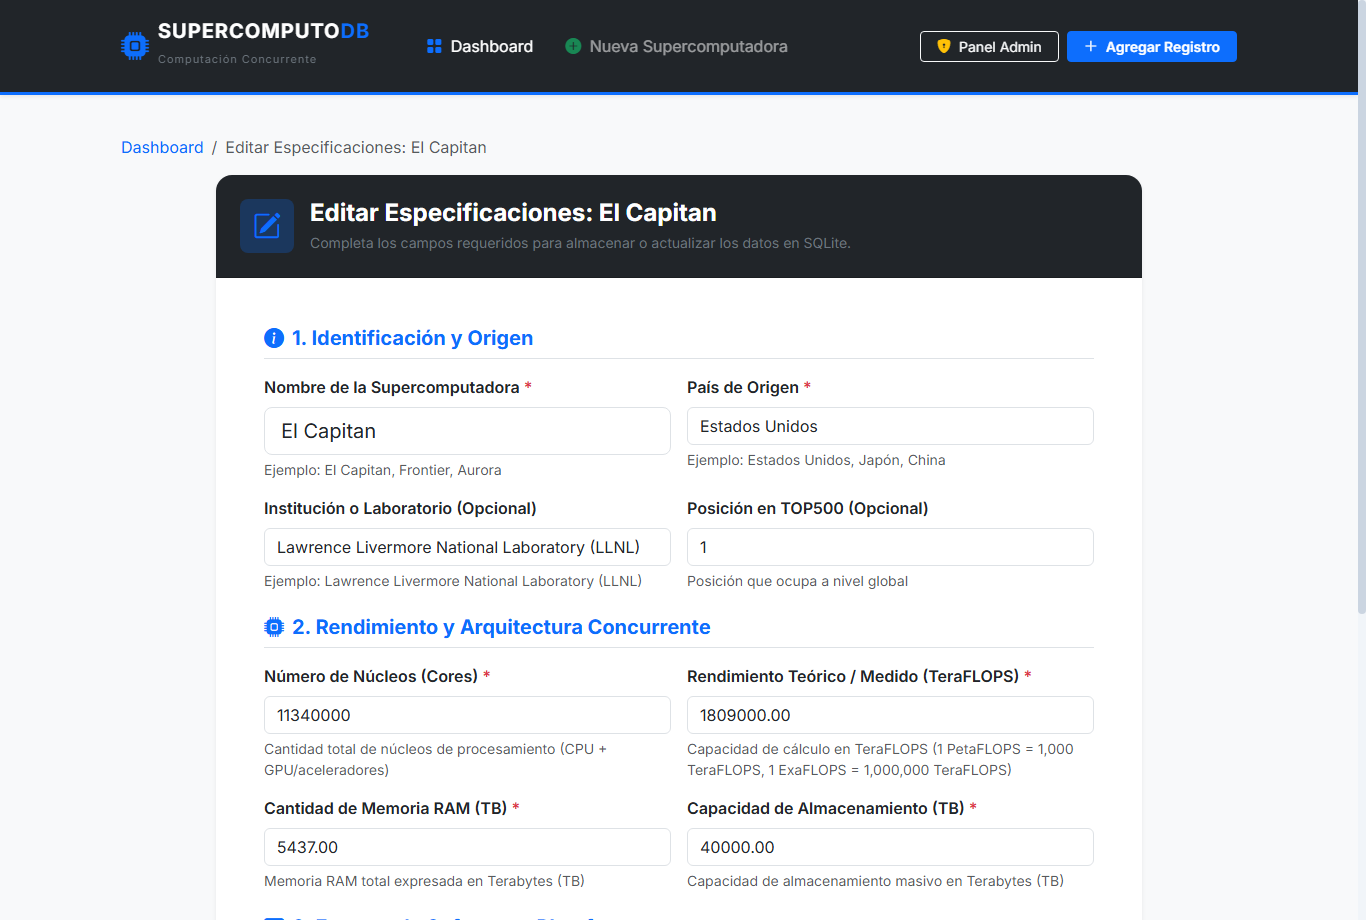
\includegraphics[width=0.95\textwidth]{imagenes/13_web_editar_formulario.png}
    \caption{Formulario de edición con información precargada lista para su modificación.}
    \label{fig:web_edit}
\end{figure}

\newpage
\subsection{5. Función Borrar: Eliminación Segura con Confirmación}
Para evitar pérdidas accidentales de información en SQLite, la ruta \texttt{/<id>/eliminar/} requiere confirmación explícita mediante un método HTTP \texttt{POST} protegido con token CSRF, impidiendo ataques de tipo Cross-Site Request Forgery.

\begin{figure}[H]
    \centering
    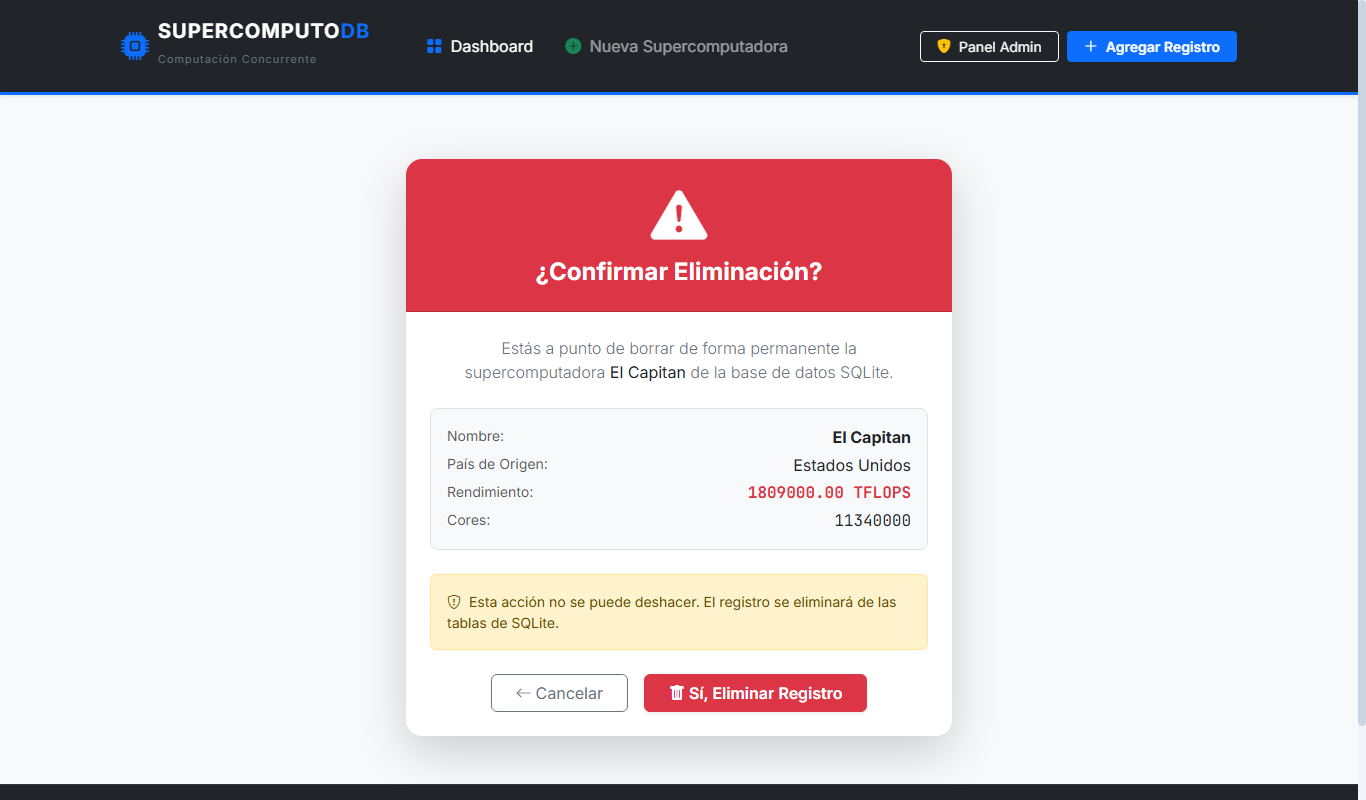
\includegraphics[width=0.88\textwidth]{imagenes/14_web_confirmar_eliminar.png}
    \caption{Pantalla de confirmación previa a la eliminación física del registro en la base de datos.}
    \label{fig:web_del}
\end{figure}

\newpage
\subsection{6. Panel Administrativo Oficial de Django}
Se configuró la integración con el módulo administrativo nativo (\texttt{/admin/}), el cual proporciona capacidades de búsqueda de texto completo, filtros laterales por país y sistema operativo, y registro de auditoría de modificaciones.

\begin{figure}[H]
    \centering
    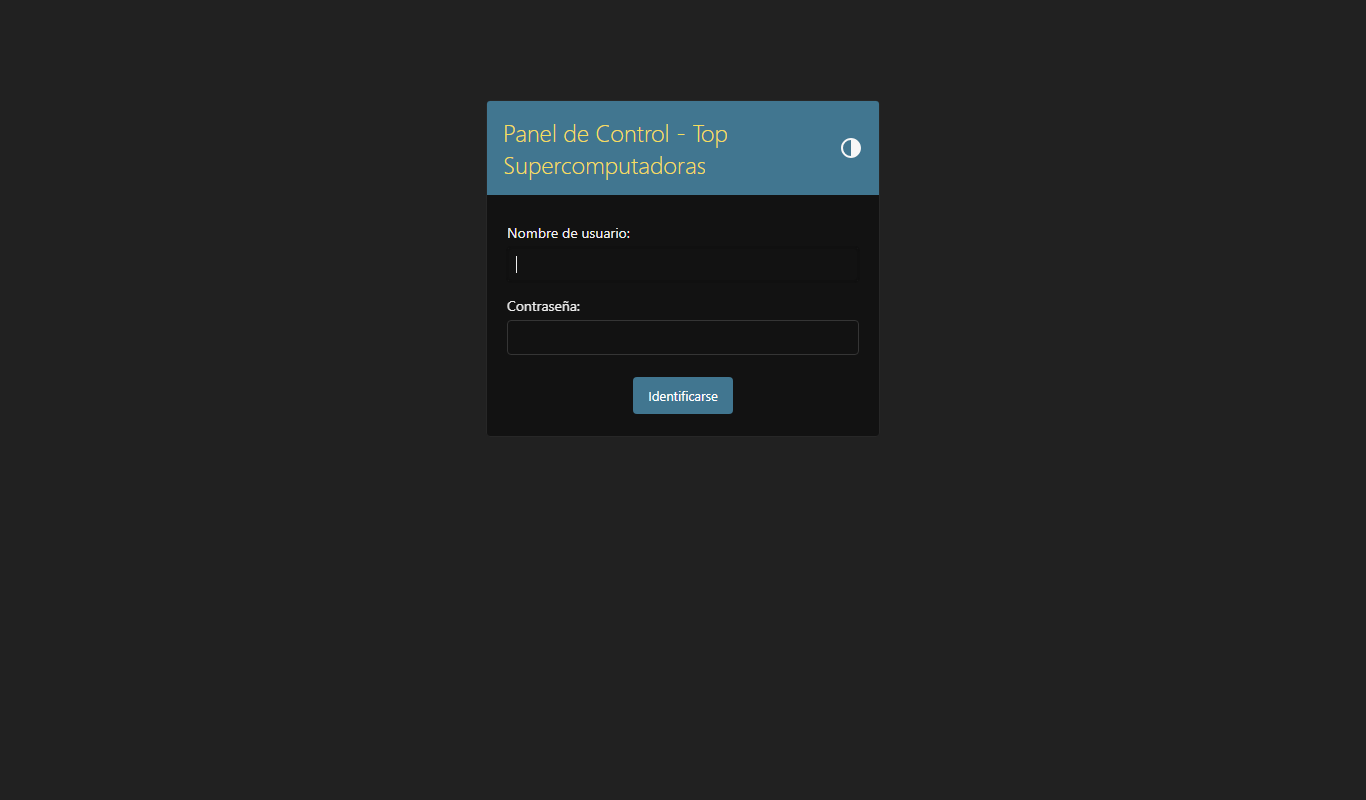
\includegraphics[width=0.92\textwidth]{imagenes/15_web_admin_login.png}
    \caption{Pantalla de autenticación para el panel administrativo oficial de Django.}
    \label{fig:admin_login}
\end{figure}

\begin{figure}[H]
    \centering
    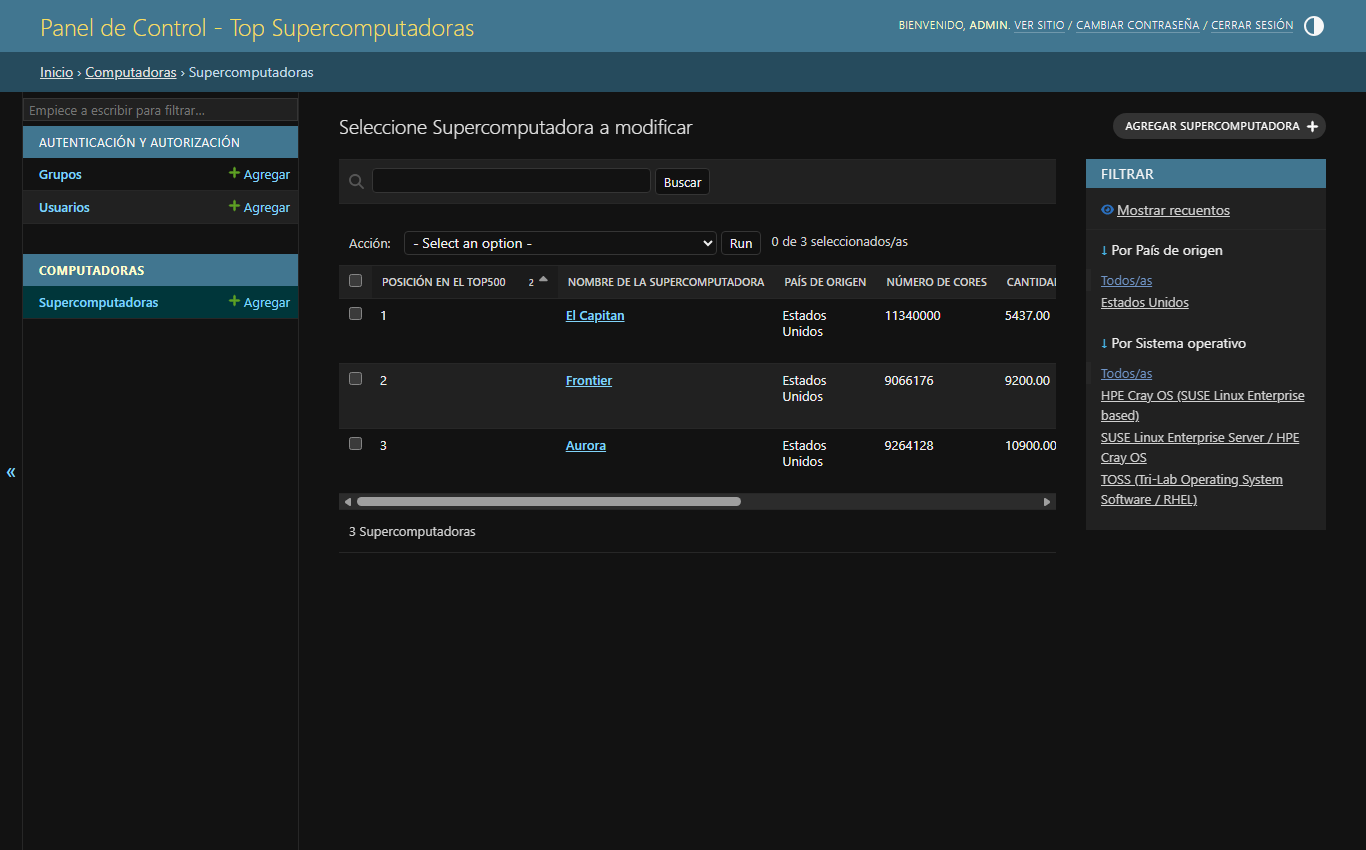
\includegraphics[width=0.95\textwidth]{imagenes/16_web_admin_listado.png}
    \caption{Panel administrativo con vista tabular, filtros avanzados y buscador de registros.}
    \label{fig:admin_list}
\end{figure}

\newpage

% =========================================================================
% SECCIÓN 6: CÓDIGO FUENTE CLAVE EXPLICADO
% =========================================================================
\section{Implementación del Código Fuente}

A continuación se analizan los fragmentos de código centrales que dan sustento a la persistencia de datos y a la lógica web de la aplicación.

\subsection{1. Modelo de Datos: \texttt{computadoras/models.py}}
El modelo declara la estructura de la tabla relacional, aplicando restricciones de unicidad y validadores de rango positivo.

\begin{lstlisting}[language=Python, caption={Modelo Supercomputadora en models.py}]
from django.db import models
from django.urls import reverse
from django.core.validators import MinValueValidator

class Supercomputadora(models.Model):
    # 1. Nombre de la supercomputadora (unico)
    nombre = models.CharField(max_length=120, unique=True, verbose_name="Nombre")
    
    # 2. Pais de origen
    pais_origen = models.CharField(max_length=100, verbose_name="Pais de origen")
    
    # 3. Numero de cores concurrentes (64 bits para evitar overflow)
    numero_cores = models.PositiveBigIntegerField(
        verbose_name="Numero de cores",
        validators=[MinValueValidator(1)]
    )
    
    # 4. Memoria RAM principal en Terabytes
    ram_tb = models.DecimalField(
        max_digits=12, decimal_places=2,
        verbose_name="RAM (TB)",
        validators=[MinValueValidator(0.01)]
    )
    
    # 5. Capacidad de almacenamiento en Terabytes
    almacenamiento_tb = models.DecimalField(
        max_digits=14, decimal_places=2,
        verbose_name="Almacenamiento (TB)",
        validators=[MinValueValidator(0.01)]
    )
    
    # 6. Rendimiento en TeraFLOPS (precision decimal exacta)
    teraflops = models.DecimalField(
        max_digits=16, decimal_places=2,
        verbose_name="Rendimiento (TeraFLOPS)",
        validators=[MinValueValidator(0.01)]
    )
    
    # 7. Sistema operativo base
    sistema_operativo = models.CharField(max_length=150, verbose_name="Sistema operativo")

    # Campos complementarios de apoyo
    fabricante = models.CharField(max_length=150, blank=True)
    institucion = models.CharField(max_length=180, blank=True)
    ranking_posicion = models.PositiveIntegerField(null=True, blank=True)
    fecha_registro = models.DateTimeField(auto_now_add=True)
    fecha_actualizacion = models.DateTimeField(auto_now=True)

    class Meta:
        ordering = ["-teraflops", "ranking_posicion", "nombre"]

    def __str__(self):
        return f"{self.nombre} ({self.pais_origen}) - {self.teraflops:,.2f} TFLOPS"

    # Conversiones calculadas dinamicamente
    @property
    def petaflops(self):
        return float(self.teraflops) / 1000.0

    @property
    def exaflops(self):
        return float(self.teraflops) / 1_000_000.0

    @property
    def ram_petabytes(self):
        return float(self.ram_tb) / 1000.0

    @property
    def almacenamiento_petabytes(self):
        return float(self.almacenamiento_tb) / 1000.0
\end{lstlisting}

\subsection{2. Vistas del CRUD: \texttt{computadoras/views.py}}
La lógica de negocio se implementó mediante vistas genéricas basadas en clases (\textit{Class-Based Views}), lo cual reduce la duplicación de código (\textit{DRY}) y estandariza el manejo de formularios y redirecciones.

\begin{lstlisting}[language=Python, caption={Vistas genericas del CRUD en views.py}]
from django.urls import reverse_lazy
from django.contrib import messages
from django.views.generic import ListView, DetailView, CreateView, UpdateView, DeleteView
from django.db.models import Sum, Count
from .models import Supercomputadora
from .forms import SupercomputadoraForm

class SupercomputadoraListView(ListView):
    model = Supercomputadora
    template_name = "computadoras/lista.html"
    context_object_name = "supercomputadoras"

    def get_context_data(self, **kwargs):
        ctx = super().get_context_data(**kwargs)
        # Sumarizacion de recursos concurrentes directo en SQLite
        ctx["stats"] = Supercomputadora.objects.aggregate(
            total_equipos=Count("id"),
            total_cores=Sum("numero_cores"),
            total_ram=Sum("ram_tb"),
            total_almacenamiento=Sum("almacenamiento_tb"),
            total_teraflops=Sum("teraflops"),
        )
        return ctx

class SupercomputadoraDetailView(DetailView):
    model = Supercomputadora
    template_name = "computadoras/detalle.html"
    context_object_name = "computadora"

class SupercomputadoraCreateView(CreateView):
    model = Supercomputadora
    form_class = SupercomputadoraForm
    template_name = "computadoras/formulario.html"
    success_url = reverse_lazy("computadoras:lista")

    def form_valid(self, form):
        messages.success(self.request, f"Equipo '{form.cleaned_data['nombre']}' registrado con exito.")
        return super().form_valid(form)

class SupercomputadoraUpdateView(UpdateView):
    model = Supercomputadora
    form_class = SupercomputadoraForm
    template_name = "computadoras/formulario.html"
    success_url = reverse_lazy("computadoras:lista")

    def form_valid(self, form):
        messages.info(self.request, f"Registro '{form.cleaned_data['nombre']}' actualizado.")
        return super().form_valid(form)

class SupercomputadoraDeleteView(DeleteView):
    model = Supercomputadora
    template_name = "computadoras/confirmar_eliminar.html"
    context_object_name = "computadora"
    success_url = reverse_lazy("computadoras:lista")
\end{lstlisting}

\newpage
\subsection{3. Enrutamiento de URLs: \texttt{computadoras/urls.py}}
Las rutas se configuran mediante identificadores semánticos y parámetros tipificados (\texttt{<int:pk>}), lo que permite vincular las vistas con las plantillas de forma modular.

\begin{lstlisting}[language=Python, caption={Definicion de rutas URL de la aplicacion}]
from django.urls import path
from . import views

app_name = "computadoras"

urlpatterns = [
    path("", views.SupercomputadoraListView.as_view(), name="lista"),
    path("<int:pk>/", views.SupercomputadoraDetailView.as_view(), name="detalle"),
    path("nueva/", views.SupercomputadoraCreateView.as_view(), name="crear"),
    path("<int:pk>/editar/", views.SupercomputadoraUpdateView.as_view(), name="editar"),
    path("<int:pk>/eliminar/", views.SupercomputadoraDeleteView.as_view(), name="eliminar"),
]
\end{lstlisting}

% =========================================================================
% SECCIÓN 7: CONCLUSIONES Y REFERENCIAS
% =========================================================================
\section{Conclusiones Técnicas y Referencias}

\subsection{Conclusiones del Proyecto}
\begin{enumerate}
    \item \textbf{Dimensión de la Concurrencia en Supercómputo:} Analizar las especificaciones de \textit{El Capitan}, \textit{Frontier} y \textit{Aurora} permitió comprender que la concurrencia moderna a exaescala ya no depende únicamente del incremento en la frecuencia de reloj, sino de la integración masiva de núcleos heterogéneos (CPU + aceleradores) interconectados con memorias de altísimo ancho de banda (HBM3) y redes de baja latencia (Slingshot-11).
    \item \textbf{Evaluación de Concurrencia en SQLite:} Se constató que SQLite es una solución sumamente ágil y adecuada para proyectos de investigación y aplicaciones de escala departamental. Gracias a su mecanismo de cerrojos compartidos, permite lecturas simultáneas eficientes sin sobrecarga administrativa. Para escenarios de producción con cientos de escrituras simultáneas por segundo, la serialización impuesta por su cerrojo exclusivo aconsejaría la transición hacia un motor como PostgreSQL con control de concurrencia multiversión (MVCC).
    \item \textbf{Solidez y Mantenibilidad con Django:} El patrón MVT y el uso de vistas basadas en clases facilitaron una implementación limpia de las cuatro operaciones CRUD solicitadas, garantizando validaciones estrictas y protección nativa contra inyecciones SQL y ataques CSRF.
\end{enumerate}

\subsection{Referencias Bibliográficas y Enlaces Consultados}
\begin{itemize}
    \item \textbf{TOP500 Supercomputers Project:} Ranking oficial de supercómputo mundial. \url{https://top500.org/}
    \item \textbf{Documentación Oficial de Django:} Framework web en Python. \url{https://docs.djangoproject.com/}
    \item \textbf{SQLite Documentation:} File locking and concurrency in SQLite 3. \url{https://www.sqlite.org/lockingv3.html}
    \item \textbf{Visual Studio Code:} Entorno de desarrollo integrado. \url{https://code.visualstudio.com/}
    \item \textbf{¿Qué es Django y por qué importa? - Django y DRF:} \url{https://www.youtube.com/watch?v=B8OlRdYwNlA}
    \item \textbf{Django Portafolio, Ejemplo Práctico:} \url{https://www.youtube.com/watch?v=zBjMF6je24U}
    \item \textbf{Django REST Framework y React CRUD:} \url{https://www.youtube.com/watch?v=38XWpyEK8IY}
    \item \textbf{Crea una agenda virtual con Django:} \url{https://www.youtube.com/watch?v=EQ-kqDmfUoM}
\end{itemize}

\end{document}
